\documentclass{amsart}
\usepackage{graphicx} % Required for inserting images
\usepackage{amssymb}
\usepackage{verbatim}
\usepackage{hyperref}
\usepackage{mathtools}
\usepackage{bbm}
\usepackage{enumerate}

\usepackage{xy}
\xyoption{all}

% \usepackage{tikz}
% \usetikzlibrary{arrows.meta}

%%%%%%%%%%%%% FORMATTING %%%%%%%%%%%%%

% Spacing
\usepackage{setspace}
\singlespacing


% Margins, etc
\usepackage{geometry} 

% Saving title space
\geometry{a4paper, margin=1in}
\usepackage{titling}
\setlength{\droptitle}{0em}

% Custom footer
\usepackage{fancyhdr}
\pagestyle{fancy}
\lhead{Caleb Hill}
\rhead{UNH Mathematics}
\lfoot{  }
\rfoot{  }

% Bibliography
\usepackage[
backend=biber,
style=numeric,
% style=authoryear
% style=bwl-FU
]{biblatex}
\addbibresource{refs.bib}



%%%%%%%%%%%%%%%%% MARKUPS %%%%%%%%%%%%%%%%%%%%%%%
\usepackage[color=cyan]{todonotes}
\usepackage{color}
\newcommand{\red}[1]{{\color{red}{#1}}}
\newcommand{\blue}[1]{{\color{blue}{#1}}}
\newcommand{\cainsays}[1]{\blue{Cain says: #1}}



%%%%%%%%%%%%%%%%%% MATH %%%%%%%%%%%%%%%%%%%%%%

\newcommand{\onto}{\twoheadrightarrow}

\newcommand{\N}{\mathbb{N}}
\newcommand{\Z}{\mathbb{Z}}
\newcommand{\Q}{\mathbb{Q}}
\newcommand{\R}{\mathbb{R}}
\newcommand{\C}{\mathbb{C}}
\newcommand{\unit}{\mathbbm{1}} % depends on package bbm

\newcommand{\CC}{\mathcal{C}}
\newcommand{\DD}{\mathcal{D}}
\newcommand{\EE}{\mathcal{E}}
\newcommand{\FF}{\mathcal{F}}
\newcommand{\GG}{\mathcal{G}}
\newcommand{\MM}{\mathcal{M}}
\newcommand{\PP}{\mathcal{P}}
\newcommand{\Neg}{\mathcal{N}}

\newcommand{\tr}{tr}
\newcommand{\id}{id}
\newcommand{\ldag}{\langle}
\newcommand{\rdag}{\rangle^\dagger}
\newcommand{\ol}{\overline}

\newcommand{\dd}{\mathfrak{d}}
\newcommand{\ee}{\mathfrak{e}}
\renewcommand{\gg}{\mathfrak{g}}
\newcommand{\hh}{\mathfrak{h}}
\renewcommand{\sl}{\mathfrak{sl}}
\newcommand{\cat}[1]{\ol{\Rep(U_{#1}(\gg_2))}}

\DeclareMathOperator{\ob}{ob}
\DeclareMathOperator{\im}{im}
\DeclareMathOperator{\Rep}{Rep}
\DeclareMathOperator{\Hom}{Hom}
\DeclareMathOperator{\Alg}{Alg}
\DeclareMathOperator{\GPA}{GPA}
\DeclareMathOperator{\End}{End}
\DeclareMathOperator{\Vecc}{Vec}
\DeclareMathOperator{\Sym}{Sym}
\DeclareMathOperator{\Kar}{Kar}
\DeclareMathOperator{\ev}{ev}
\DeclareMathOperator{\coev}{coev}
\DeclareMathOperator{\Res}{Res}
\DeclareMathOperator{\Ab}{Ab}


\renewcommand{\phi}{\varphi}
\let\oldepsilon\epsilon\let\epsilon\varepsilon\let\smallepsilon\oldepsilon %this makes \epsilon produce the curly epsilon, and \smallepsilon the smaller epsilon

\newcommand{\blank}{\rule{0.2cm}{0.15mm}}


\newcommand{\codebasename}{\texttt{OTimes}}


%%%%%%%%%%%%%%%%%% THEOREMS %%%%%%%%%%%%%%%%%%%%%%
\theoremstyle{plain}
    \newtheorem{definition}{Definition}
    \newtheorem{example}{Example}
    \newtheorem{proposition}{Proposition}
    \newtheorem{theorem}{Theorem}
    \newtheorem{lemma}{Lemma}
    \newtheorem{corollary}{Corollary}
    \newtheorem{conjecture}{Conjecture}
    \newtheorem{remark}{Remark}



% skein diagrams
\newcommand{\skein}[2]{\raisebox{-.4\height}{ \includegraphics[scale = #2]{figs/#1.png}}}


\title{Quantum Subgroups of $G_2$ via Graph Planar Algebra Embeddings}
\author{Caleb Kennedy Hill}
\date{}

\begin{document}
\maketitle



\red{
Cain's notes
\begin{itemize}
    \item Show off $\DD_i$ in the intro. Theorem: skein cats like this exist
    \item don't oversell and say ``these will be of great use.'' Define and then show utility.
    \item Delete lots of prelim material. Just cite.
    \item Delete final proof. Cite Cain and Noah
    \item Overall style not academic enough. Dry it out.
    \item relns might lead to zero
\end{itemize}

}




% \tableofcontents


% \section{Introduction}

This paper gives generators-and-relations presentations for two categories 
\[
    \cat{q_3}_{A_3} \quad \text{and} \quad \cat{q_4}_{A_4}
\] 
where $A_3$ and $A_4$ are the commutative Etale algebras corresponding, respectively, 
to the conformal embeddings $G_{2,3} \subseteq E_{6,1}$ and $G_{2,4} \subseteq D_{7,1}$ 
of affine Lie algebras. 
The correspondence $\CC(\gg,k) \xleftrightarrow{} \ol{\Rep(U_{q_k}(\hh))}$ between 
affine Lie algebra representations and quantum group representations \red{need citation} allows one, 
in the course of studying conformal embeddings, to move freely from the perspective of 
affine Lie algebras to that of quantum groups. 
We will initialize our statements in the language of affine Lie algebras, 
and then translate into quantum groups.

By {\it presentation} we mean the following standard sequence of steps. 
Let $\PP$ be the planar algebra generated by some object of the tensor category $\CC$. 
Then we show $\PP$ is monoidally equivalent to some skein category $\EE$, and that $\Ab(\EE)$ is monoidally equivalent to $\CC$. 
The presentations we give are extensions of Kuperberg's $\GG_2(q)$ skein theory by strands of type $\Z_3$ (level 3) and $\Z_2$ (level 4). 

The novel methodology offered here is the use of graph planar algebra (GPA) embeddings to deduce relations. 
Computing, e.g., the relation (Change of Basis) purely in the context of quantum group representations is daunting, to say the least. 
With a GPA embedding in hand, however, this becomes an elementary linear algebra problem. 
This approach is counter to the usual approach take by, say, Copeland and Edie-Michell in \cite{Cain_Dan}.
Those authors move from generators-and-relations presentations to GPA embeddings for the purpose of 
constructing module categories over $\ol{\Rep(U_q(\sl_N))}$ categories.

Even work with the same aim as this paper, e.g., presenting categories $\CC_A$ of algebras has, thus far,
taken a markedly different form.
The closest example is the recent work of Edie-Michell and Snyder \cite{cain_noah_hans}, which gives presentations 
for categories of the form $\ol{\Rep(U_q(\sl_N))}_A$.
The methods used by these authors is purely representation theoretic;
that is, all of the skein relations for those categories can be deduced from first principles.
At this time there seems to be no clear path from pure representation theory to the presentations we give.
More tools are needed.
Enter GPA embeddings.

% Harder than cain and noah's case becasue I needed to find more relns.
% So this uses GPA emb to find more relns

The present work is organized as follows.
Section~\ref{sec:prelim} sets up most of the theory needed, referencing that which we do not exposit here.
This includes unoriented planar algebras, unoriented graph planar algebras, 
internal algebra and module objects, and some assorted theoretical devices and results.
Section~\ref{sec:skein} then goes on to define a general class of categories of which our examples are members.
We expect this class of categories to be of great use for those researchers intent on conjuring 
examples of exotic new tensor categories.
We then show this class of categories to be evaluable.
Section~\ref{sec:methods} then goes on to discuss what the details of the process of using GPA 
embeddings looks like.
Subsection~\ref{subsec:triv-vertex} details the techniques used to arrive at GPA embeddigns of 
trivalent categories. 
Subsection~\ref{subsec:proj-relns} shows how we go beyond these embeddings of trivalent categories,
and how we use GPA embeddings to explore relations in extensions of trivalent categories.
Finally, Sections~\ref{sec:results-3} and \ref{sec:results-4} give the structure constants for the 
newly constructed categories.
Section~\ref{sec:results-3} details the argument used to prove that we truly have found full presentations.
This covariant Galois-esque argument also appears in \cite{cain_noah_hans}.
\section{Introduction}\label{sec:intro}
Quantum subgroups are a well-known source of tensor categories.
More precisely, given a conformal embedding $\VV(\gg,k) \subseteq \VV(\hh,1)$ of VOAs 
as in \cite{DMNO}, one obtains a corresponding Etale algebra $A$.
This algebra then allows one to consider the category $\ol{\Rep(U_q(\gg))}_A$ of right $A$-modules.
A half-braiding on $A$ then gives a tensor product on $\ol{\Rep(U_q(\gg))}_A$, and one may study this
new category in its own right.
The free functor gives an embedding $\ol{\Rep(U_q(\gg))} \hookrightarrow \ol{\Rep(U_q(\gg))}_A$.
As this embedding is, in general, not full, it remains only to 
find a description of the new morphisms in $\ol{\Rep(U_q(\gg))}_A$.
Recent works of Edie-Michell and Snyder \cite{cain_noah} have used this reasoning, and 
representation theoretic techniques to give diagrammatic descriptions of new tensor categories of modules
corresponding to the family of conformal embeddings $\VV(\sl_N,N^2) \subseteq \VV(\sl_{N^2-1},1)$.

On the other hand, one may start with a known category and compute graph planar algebra (GPA) embeddings for it.
This has been done for $\ol{\Rep(U_q(\sl_N))}$ in \cite{Cain_Dan} and for the 
extended Haagerup categories in \cite{extended_haagerup}.
This computation has the theoretical and practical consequences.
By the GPA embedding theorem \cite{something}, such an embedding immediately gives a module category.
It additionally gives a concrete representation of the category in which one may perform explicit computations.

The present work describes a blend of these two techniques.
We begin by fidning a GPA embedding on the well-known trivalent category $\GG_2(q)$ of \cite{Kuperberg,tricats}
which is a diagrammatic presentation for $\ol{\Rep(U_q(\gg_2))}$.
Through the free fucntor we can view our GPA embedding as a GPA embedding for a $\otimes$-generating 
object's planar algebra in $\ol{\Rep(U_q(\gg_2))}_A$.
This gives us a black-strand.
We then search inside the GPA embedding for new morphisms.
According to \cite{DMNO} there ought to be a projection onto a $\Z_k$-like simple object in $\ol{\Rep(U_q(\gg_2))}_A$,
so this is what we search for inside the GPA.
We view this new morphism as an orange strand.
The properties of this new morphism are unknown beyond a scant basic set.
Once we have or hands on the imagine in the GPA of this projection, though, 
we may explore its properties through explicit computations.
We perform this process of extending GPA embeddings for the two conformal embeddings
\begin{equation}\label{eq:conf-embs}
    \VV(\gg_2,3) \subseteq \VV(\ee_6,1) \quad\text{and}\quad \VV(\gg_2,4) \subseteq \VV(\dd_7,1).
\end{equation}

Now we begin by introducing some notation for a skein theory involving an oritned, colored strand 
in addition to unoriented black strands.
\begin{definition}
    For a diagram $\EE$ the notation $r^i(\EE)$ means an $i$-click right rotation. 
    For instance, 
    \[
    r^1\left( \skein{/skein_figs/doubleStick}{0.07} \right) = \skein{/skein_figs/capcup}{0.07} 
    \quad\text{and}\quad 
    r^2\left( \skein{/skein_figs/doubleStick}{0.07} \right) = \skein{/skein_figs/doubleStick}{0.07}.
    \] 

    Suppose the diagram $\EE$ has $m$ boundary points. 
    We define $dec_i(\EE)$ to be the $i$-th external single clockwise decoration of $\EE$. 
    For example,
    \[
        dec_1\left(\skein{/skein_figs/trivalent}{0.15}\right) = \skein{/skein_figs/rightDown}{0.1},
    \quad
    \text{and} 
    \quad
        \sum_{i=1}^{3} dec_i\left(\skein{/skein_figs/trivalent}{0.15}\right) 
        = \skein{/skein_figs/rightDown}{0.1} 
        +v\skein{/skein_figs/bottomLeft}{0.1} 
        +v\skein{/skein_figs/leftUp}{0.1}
    \]
    We adopt the convention that $dec_0 (\EE) = \EE$.
\end{definition}

Both of the categories studied in this paper are extensions of trivalent categories by a colored, directed, $\Z_n$-like strand. 
We define the class of categories we will be working with.
In Section~\ref{sec:skein} we will show that, with an assumption on the underlying skein theory, 
categories in this class are evaluable in general.
\begin{definition}\label{def:zn-ext}
    Let $\CC = \left\langle \skein{/skein_figs/trivalent}{0.1} \right\rangle$ 
    be a trivalent category. 
    Call $\DD$ a {\bf $\Z_n$-like extension} of $\CC$ if we have
    $\DD = \left\langle \skein{/skein_figs/trivalent}{0.1}, \skein{/skein_figs/Pg}{0.1} \right\rangle$,
    enjoying the following relations\footnote{Conditions from \cite{czenky}.}:
    \begin{equation*}\tag{Recouple}
        \skein{/skein_figs/recouple_LHS}{0.1} 
        = c \skein{/skein_figs/recouple_RHS}{0.1}
    \end{equation*}

    \begin{equation*}\tag{\red{Reverse}}
        \skein{/skein_figs/recouple_LHS}{0.1} 
        = c \skein{/skein_figs/recouple_RHS}{0.1}
    \end{equation*}

    \begin{equation*}\tag{Schur 0}
        \skein{/skein_figs/schur_0_1}{0.1} = 0 \quad 
        \skein{/skein_figs/schur_0_2}{0.1} = 0 \quad \cdots \quad 
        \underbrace{ \skein{/skein_figs/schur_0_n-1}{0.11} }_{\text{$n-1$}} = 0
    \end{equation*}

    \begin{equation*}\tag{Schur 1}
        \skein{/skein_figs/schur_1_1}{0.1} = 0 \quad 
        \skein{/skein_figs/schur_1_2}{0.1} = 0 \quad \cdots \quad 
        \underbrace{ \skein{/skein_figs/schur_1_n-1}{0.11} }_{\text{$n-1$}} = 0
    \end{equation*}

    \begin{equation*}\tag{Swap}
        \skein{/skein_figs/swap_LHS}{0.15} 
        = \omega \skein{/skein_figs/swap_RHS}{0.15}
    \end{equation*}

    \begin{equation*}\tag{decStick}
        \skein{/skein_figs/stick_w_Pg}{0.25} 
        = a \skein{/skein_figs/stick}{0.1}
    \end{equation*}

    \begin{equation*}\tag{decBigon}
        \skein{/skein_figs/g_bigon2}{0.1} = b \skein{/skein_figs/stick}{0.15}
    \end{equation*}

    \begin{equation*}\tag{Change of Basis}
        \skein{/skein_figs/leftUp}{0.1} 
        = \sum_{i=0}^{n-1} r_i \skein{/skein_figs/rightUp}{0.1}^i
    \end{equation*}

    \begin{equation*}\tag{decTrigon}
        \skein{/skein_figs/trigon_singly}{0.1} 
        = \sum_{i=0}^{n-1} t_i \skein{/skein_figs/rightUp}{0.1}^i
    \end{equation*}\label{eq:decTrigon}

    \begin{equation*}\tag{decTetragon}
         \skein{/skein_figs/square_singly}{0.12} 
         = \sum_{i=0}^4 \sum_{j=0}^3 u_{i,j} dec_i\left( r^j\left( \skein{/skein_figs/eye_map}{0.1} \right) \right)
         + \sum_{i=0}^4 \sum_{j=0}^3 v_{i,j} dec_i\left( r^j\left( \skein{/skein_figs/doubleStick}{0.1} \right) \right)
    \end{equation*}

     \begin{equation*}\tag{decPentagon}
        \skein{/skein_figs/pentagon_singly}{0.17} 
        = \sum_{i=0}^5 \sum_{j=0}^4 w_{i,j} dec_i\left( r^j\left( \skein{/skein_figs/pent_1}{0.2} \right) \right) 
        + \sum_{i=0}^5 \sum_{j=0}^4 x_{i,j} dec_i\left( r^j\left( \skein{/skein_figs/pent_2}{0.12} \right) \right)
    \end{equation*}
\end{definition}


\begin{proposition}
    (1) ($\Z_n$) follows from (Recouple) and (Reverse).

    (2) (Split) follows from (Recouple) and ($\Z_n$).

    \begin{equation*}\tag{Split}
        \underbrace{ \skein{/skein_figs/split_LHS}{0.125} }_{\text{$n$}} 
        = s \underbrace{ \skein{/skein_figs/split_RHS}{0.085} }_{\text{$n$}}
    \end{equation*}

    \begin{equation*}\tag{$\Z_n$}
        \underbrace{ \skein{/skein_figs/n_g_strands}{0.08} }_{\text{$n$}} 
        = z \skein{/skein_figs/capcup}{0.1}
    \end{equation*}
\end{proposition}
\begin{proof}
    (1) 

    (2) 
\end{proof}

\begin{remark}
    A quick sketch shows that using (Order) followed by repeated applications of (Recouple) and (decStick) 
    allows one to swap an up-oriented strand for $n-1$ down-oriented strand. 
    This means that, upon reversing the orientations of the lefthand sides of the relations in 
    Definition~\ref{def:zn-ext} will give similar relations.
    This fact will be used in the proof of Lemma~\ref{lem:ext-dec}.
\end{remark}


\begin{remark}
    It is worth noting the following standard abuse of language. 
    A diagrammatically presented category such as a $\Z_n$-like extension has hom-spaces which are formal spans of diagrams.
    When applying a relation such as (decTrigon) locally, the result is clearly a {\it linear combination} of diagrams.
    Usually, though, this linear combination has some desirable quality, such as a smaller number of internal faces in each summand.
    In this instance, we prefer to say something along the lines of, 
    ``applying (decTrigon) decreases the number of internal faces,''
    instead of, for instance, the more wordy,
    ``applying (decTrigon) turns this diagram into a linear combination of diagrams with fewer internal faces.''
\end{remark}



\begin{definition}
    Set $q_4 = e^{\frac{2\pi i}{48}}$ and deifne $\DD_4$ to be the $\Z_2$-like extension of $\GG_2(q_4)$ with structure constants
    \begin{equation*}
    \omega = -1
    \end{equation*}

    \begin{equation*}
        r_1 = e^{-\frac{\pi i}{6}}, \quad r_2 = e^{-\frac{2\pi i}{3}}
    \end{equation*}

    \begin{equation*}
        s_1 = e^{-\frac{\pi i}{6}} \quad s_2 = e^{-\frac{4\pi i}{3}}
    \end{equation*}

    \begin{equation*}
        t_1 = -1 \quad t_2 = -1
    \end{equation*}

    \begin{align*}
        u = 1, && u = 2, && u = 3, && u = 4, && u = 5, && u = 6, \\
        v = 7, && v = 8, && v = 9, && v = 10, && v = 11, && v = 12 
    \end{align*}


\end{definition}



One of the two primary results we give here is that $\DD_4$ is a presentation for a category of modules corresponding to the
level 4 conformal embedding of $\gg_2$.
\begin{theorem}
    There is an equivalence
    \[
        \Ab(\DD_4) \cong \ol{\Rep(U_{q_4}(\gg_2))}_{A_4}
    \]
    where $A_4$ is the algebra object corresponding to the level-4 conformal embedding of \ref{eq:conf-embs}.
\end{theorem}
Theorem~\ref{thm:level-3} is an analogous theorem for level 3, with structure constants given in the attached Mathematica files.



It is not clear a priori that the defining relations for, say, $\DD_4$ lead to a nontirivial tensor category.
The general undecidability of the word problem for groups offers some evidence that this question is difficult
for a typical presentation for a tensor category.
That is, one should not expect a set of relations to yield any nontriviality.
It follows that the presentations we give here are interesting and worth investigating more generally.

% \red{check (sub)(sub)section types}
The remainder of the paper is structured as follows.
Section~\ref{sec:prelim} sets up most of the theory needed, referencing that which we do not exposit here.
This includes unoriented planar algebras, unoriented graph planar algebras, 
internal algebra and module objects, and some assorted theoretical devices and results.
Section~\ref{sec:skein} then goes on to investigate some properties of $\Z_n$-like extensions.
We expect this class of categories to be of use for researchers intent on conjuring 
examples of exotic tensor categories.
In fact, in a forthcoming paper, the present author and Cain Edie-Michell diagrammatically
present a number of near-group categories as $\Z_n$-like extensions of $SO(3)_q$ trivalent categories.
We demonstrate evaluability of this class of catgeories under a relatively tame assumption on the
underlying trivalent skein theory.
Section~\ref{sec:methods} discusses the process of arriving at GPA embeddings.
Subsection~\ref{subsec:triv-vertex} details the techniques used to arrive at GPA embeddigns of 
trivalent categories. 
Subsection~\ref{subsec:proj-relns} shows how we extend these embeddings of trivalent categories
to embeddings of $\Z_n$-like extensions, and how we use GPA embeddings to explore 
relations in these extensions.
This section uses examples from level 4 ($\DD_4$) due to the fact that the numbers involved are more presentable.
The process used for level 3 ($\DD_3$) was essentially identical.
Finally, Section~\ref{sec:results} gives the structure constants for the newly constructed categories.
This section also discusses the argument used to prove that we truly have found full presentations.
The argument appears in its entirety in \cite{cain_noah}, and is adapted to the present settign without a problem.

\section{Preliminaries}\label{sec:prelim}
Here we define the players in this game. We begin with planar algebras, in the spirit of \cite{tricats}.



\subsection{Unoriented Planar Algebras}

We begin by recalling the theory of {\bf rigid} monoidal categories detailed in \cite{KW}. 
To put it succintly, rigid monoidal categories have duals. 
Duals, and the associated evaluation and coevaluation maps, give us the cups and caps ubiquitous in planar algebras. 
A rigidity assumption gives us the ability to isotope diagrams. 
The generators we will use for our planar algebras will be symmetrically self-dual.
We also assume pivotality throughout.

Let $X$ be a (symmetrically self-dual) tensor generator for the tensor category $\CC$; 
that is, every object of $\CC$ is isomorphic to a subobject of some tensor power $X^{\otimes n}$. 
Let $\PP_{X;\CC}$ be the full subcategory of $\CC$ whose objects are tensor powers $\unit=X^{\otimes0},X,X^{\otimes2},\dots$; 
we call this the (unoriented) {\bf planar algebra} generated by $X$ in $\CC$. 
Since we assumed $X$ tensor generates $\CC$, it follows that $\CC \cong \Ab(\PP_{X;\CC})$, 
the abelian envelope of $\PP_{X;\CC}$. 
The universal property of $\Ab(\PP_{X;\CC})$ therefore implies 
that studying $\PP_{X;\CC}$ is sufficient to understand $\CC$. 
The planar algebra $\PP_{X;\CC}$ is {\bf evaluable} if $\dim\End_{\PP_{X;\CC}}(\unit)=1$. 

We will be presenting the our two new categories as extensions of $\GG_2(q)$ skein theories, in the spirit of Kuperberg \cite{Kuperberg}. 
Up to a rescaling by a factor of $k = \sqrt{[7]-1}$ we use the same skein theory (note the sign error in the \ref{eq:Pentagon} relation of \cite{Kuperberg}). 
That is, we define the planar algebra $\GG_2(q)$ generated by a trivalent vertex, with the skein relations 
    \begin{equation*}\tag{Loop}
        \skein{/skein_figs/loop}{0.1} = q^{10} + q^{8} + q^{2} + 1 + q^{-2} + q^{-8} + q^{-10}
    \end{equation*}

    \begin{equation*}\tag{Lollipop}\label{eq:Lolli}
        \skein{/skein_figs/lollipop}{0.1} = 0  
    \end{equation*}

    \begin{equation*}\tag{Rotate}\label{eq:Rotate}
        r\left( \skein{/skein_figs/trivalent}{0.1} \right) = \skein{/skein_figs/trivalent}{0.1}
    \end{equation*}

    \begin{equation*}\tag{Bigon}\label{eq:Bigon}
        \skein{/skein_figs/bigon}{0.1} = k^2 \skein{/skein_figs/stick}{0.1}
    \end{equation*}

    \begin{equation*}\tag{Trigon}\label{eq:Trigon}
        \skein{/skein_figs/trigon}{0.1} = -(q^4 +1+ q^{-4}) \skein{/skein_figs/trivalent}{0.15}
    \end{equation*}

    \begin{equation*}\tag{Tetragon}\label{eq:Tetragon}
        \skein{/skein_figs/square}{0.1} = (q^2 + q^{-2}) \left( \skein{/skein_figs/eye_map}{0.1} + \skein{/skein_figs/eye_rot}{0.1} \right) + (q^2 +1+ q^{-2}) \left( \skein{/skein_figs/capcup}{0.1} + \skein{/skein_figs/doubleStick}{0.1} \right)
    \end{equation*}

    \begin{equation*}\tag{Pentagon}\label{eq:Pentagon}
        \skein{/skein_figs/pentagon}{0.1} = - \sum_{i=0}^4 r^i \left( \skein{/skein_figs/pent_1}{0.15} \right) - \sum_{i=0}^4 r^i \left( \skein{/skein_figs/pent_2}{0.1} \right)
    \end{equation*}
Here, the notation $r^i(\EE)$ means an $i$-click right rotation of the diagram $\EE$. 
For instance, 
\[
r^1\left( \skein{/skein_figs/doubleStick}{0.07} \right) = \skein{/skein_figs/capcup}{0.07} 
\quad\text{and}\quad 
r^2\left( \skein{/skein_figs/doubleStick}{0.07} \right) = \skein{/skein_figs/doubleStick}{0.07}.
\] 
The value of $q$ is given in \cite{cain_autoequivalences} and depends on the level $k$:
\[
q = e^{\frac{2\pi i}{3(4+k)}}.
\]
Thus at level 3 we have $q_3 = e^{\frac{2\pi i}{42}}$ and at level 4 we have $q_4 = e^{\frac{2\pi i}{48}}$.




\subsection{Unitarity and inner products}
Recall that a {\bf dagger} category is one endowed with an involution, denoted by a superscript $\dagger$.
The dagger operation gives us the useful ability to reverse any morphism.
This will be of use when, for example, we need a way to pair parallel {\it or} antiparallel morphisms.

The categorical trace of a morphism $f:X\to X$  is defined by
\[
\tr(f)\coloneqq ev_{X} \circ (f\otimes \id_{X^*}) \circ coev_{X}.
\]
Informally, the trace ``caps off'' an endomorphism and returns the resulting scalar (since we assume $\dim\Hom(\unit\to\unit)\cong\C$).

We use trace to define two different notions of pairing of morphisms:
\[
\ldag f, g\rdag \coloneqq \tr(g^\dagger \circ f)
\]
for parallel morphisms and
\[
\langle \phi,\psi \rangle \coloneqq \tr(\psi\circ\phi)
\]
for antiparallel morphisms. 

Unitarity gives two tools. 
Computationally, it allows us to do computations by ``capping'' diagrams.
It also has useful theoretical consequences.
\begin{definition}
A category $\CC$ is {\bf unitary} if it is a dagger category and the two conditions
\begin{itemize}
    \item if $\ldag f,f\rdag=0$, then $f=0$
    \item for every $f:X\to Y$, there is some $g:X\to X$ such that $ff^\dagger=gg^\dagger$
\end{itemize}
are satisfied.
\end{definition}
On a related note, we also make the following definition
\begin{definition}
A morphism $f:X\to Y$ in a dagger category $\CC$ is {\bf negligible} if $\langle f,g\rangle=0$ for all $g:Y\to X$.
\end{definition}
It is a fact that the negigible morphisms in a category $\CC$ form an ideal, called the {\bf negligible idea} and denoted by $\Neg(\CC)$. We may form the semisimple quotient $\ol{\CC}\coloneqq \CC/\Neg(\CC)$.

\begin{proposition}\label{prop:negligible-induced-functor}
Let $\CC$ and $\DD$ be pivotal, with $\DD$ unitary, and $F:\CC\to\DD$ a pivotal dagger functor. 
Then $F$ descends to a faithful pivotal functor $\ol{F}:\ol{\CC}\to\DD$ such that the diagram
\[
\xymatrix@C=40pt{
\CC \ar[r]^-{F} \ar[d] & \DD \\
\ol{\CC}\ar[ur]^-{\overline{F}} &  \\
}
\]
is commutative.
\end{proposition}

\begin{proof}
    Compute directly:
    \begin{align*}
        \ldag F(f),F(f)\rdag & = \tr(F(f)^\dagger\circ F(f)) \\
        & = \tr(F(f^\dagger)\circ F(f)) \\
        & = F( \tr(f^\dagger \circ f)) \\
        & = F(0)=0
    \end{align*}
    since we assumed $f$ was negligible.
\end{proof}

As one might expect, and as was alluded to above, unitarity interacts nicely with the negligible ideal.

\begin{proposition}
    Let $\CC$ and $\DD$ be unitary, and suppose $F:\CC\to\DD$ is a pivotal dagger functor. 
    Then there is a faithful 
    $\tilde{F}:\ol{\CC} \to \ol{\DD}$
    such that
    \[
        \xymatrix@C=40pt{
        \CC \ar[r]^-{F} \ar[d] & \DD \ar[d] \\
        \ol{\CC}\ar[r]^-{\tilde{F}} & \ol{\DD}  \\
        }
    \]
    If $F$ is faithful, so is $\tilde{F}$.
\end{proposition}

\begin{proof}
    \red{ Compose $\ol{F}$ of Proposition~\ref{prop:negligible-induced-functor} with the functor $\DD \onto \ol{\DD}$. ??}
\end{proof}








\subsection{The Unoriented Graph Planar Algebra}
We will study the quantum subgroups of type $G_2$ by embedding their skein theories into appropriate graph planar algebras. This serves two purposes:
\begin{itemize}
    \item Giving us solid ground on which to do computations, allowing us to uncover relations by finding them in the GPA hom-spaces, and
    \item Implying some nice general properties for the quantum subgroups (i.e., unitarity)
\end{itemize}
In this work we have no use for generalized GPAs, such as the {\it oriented} \cite{Cain_Dan} or {\it multi-color} GPA, so we consider only the unoriented case. 

\begin{definition}\label{def:GPA}
    Let $\Gamma=(V,E)$ be a finite graph. For an edge $e=(u,v)\in E$, let $\ol{e}=(v,u)\in E$. The {\bf graph planar algebra} on $\Gamma$, denoted $\GPA(\Gamma)$, is the strictly pivotal rigid monoidal category whose objects are nonnegative integers, and whose hom-spaces have basis
    \[
        \Hom_{\GPA(\Gamma)}(m\to n) \coloneqq \C\left\{ (p,q) \mid \substack{\text{$p$ an $m$-path} \\ \text{$q$ and $n$-path}}, \substack{\text{$s(p)=s(q)$}\\ \text{$t(p)=t(q)$}} \right\},
    \]
    with composition law
    \[
        (p,q)\circ(p',q')\coloneqq \delta_{q=p'} (p,q'),
    \]
    and rigidity maps
    \[
        ev = \sum_e \sqrt{ \frac{\lambda_{t(e)}}{\lambda_{s(e)}} } \langle e\ol{e},s(e) \rangle, \quad coev = \sum_e \sqrt{ \frac{\lambda_{t(e)}}{\lambda_{s(e)}} } \langle s(e) e\ol{e} \rangle. 
    \]
    Monoidal product on objects is addition, and for morphisms is defined by 
    \[
        (p,q)\otimes(p',q')\coloneqq \delta_{s(p')=t(p)} (pp',qq').
    \]
\end{definition}


We will be finding GPA embeddings of certain planar algebras. 
The following implies unitarity of these planar algebras.
\begin{lemma}
    For $\Gamma$ a finite graph, $\GPA(\Gamma)$ is unitary.
\end{lemma}

\begin{proof}
    
\end{proof}





\subsection{Algebra and Module Objects}
Our ultimate goal is to find skein theoretic descriptions of two categories 
$\cat{q_3}_{A_3}$ and $\cat{q_4}_{A_4}$ 
of modules over algebra objects $A_3$ and $A_4$ coming from the conformal embeddings 
$\hat{\gg_2}\subseteq \hat{\ee_6}$ and $\hat{\gg_2}\subseteq \hat{\dd_7}$. 
In this subsection we define algebra and module objects. 
See \cite{ostrik2001modulecategoriesweakhopf} for a full description. 
Unless otherwise stated, we will be studying braided tensor categories.

\begin{definition}
    An {\bf algebra} object of a braided tensor category $\CC$ is an object $A$ along with two maps
    \begin{align*}
        m: & A\otimes A\to A  \\
        e: & \unit \to A  \\
    \end{align*} 
    such that the following three diagrams 
     \[
    \xymatrix@C=55pt{
    (A\otimes A)\otimes A \ar[d]^{m\otimes \id_A} \ar[r]^{a} & A\otimes(A\otimes A) \ar[r]^{\id_A \otimes m} & A\otimes A \ar[d]^{m} \\
    A\otimes A \ar[rr]^{m}  & & A\\
    }
    \] 
    and 
    \[
    \xymatrix{
    & A \ar[dl] \ar[dr] & \\
    \unit \otimes A \ar[r]^{e} \ar[dr] & A\otimes A \ar[d]^{m} & A\otimes\unit \ar[l]^{e} \ar[dl] \\
    & A & \\
    }
    \] 
    commute (where $a$ is the associator for $\CC$). Given that $\CC$ has braiding $c$, the algebra $A$ is {\bf commutative} if $m\circ c_{A,A}=m$.
    
\end{definition}


Once we have algebra objects one naturally defines modules over them.

\begin{definition}
    Given an algebra object $A$ of $\CC$, an object $M$ of $\CC$ is said to be a {\bf right $A$-module} if there is a map $s:M\otimes A\to A$ such that the diagram
    \[
    \xymatrix{
    (M\otimes A)\otimes A \ar[r]^{a} \ar[d]^{a} & M\otimes(A\otimes A) \ar[r]^{s} & M\otimes A \ar[d]^{s} \\
    M \otimes A \ar[rr]^{s} & & M \\
    }
    \]
    commutes. We define $\CC_A$ to be the category of right $A$-module objects in $\CC$.
\end{definition}
The braiding on $\CC$ allows one to give a right $A$-module the structure of a left $A$-module. Once this has been done, we may define a tensor product on $\CC_A$ by defining $M_1 \otimes_{\CC_A} M_2$ to be the pbject projected onto by the idempotent 
\[
    \skein{/skein_figs/mod_otimes}{0.19}
\]


Monoidal functors interact with algebra 
% and module 
objects in the ways we would hope.

\begin{proposition}
    Let $\FF:\CC\to\DD$ be a lax-monoidal fucntor, and let $A$ be an algebra object of $\CC$. Then $\FF A$ has algebra structure induced by $\FF$. 
    % If $M$ is a right $A$-module object of $\CC$ then $\FF M$ has a right $\FF A$-moudle structure induced by $\FF$.
\end{proposition}
\begin{proof}
    The approach is to use the lax-monoidal structure on $\FF$ and its functoriality to translate diagrams in $\CC$ to diagrams in $\DD$. See \cite{monoidalFunctorsAndAlgebras} for the full argument.
\end{proof}
The following proposition gives us license to make similar statements about adjoints of monoidal functors.
\begin{proposition}
    Monoidal functors between semisimple categories have lax-monoidal right adjoints.
\end{proposition}



The free module functor $\FF_A:\CC\to\CC_A$ given by $X\mapsto X\otimes A$ has a monoidal structure induced by the braiding on $\CC$. Its right adjoint is given by the forgetful functor $\FF^\vee:\CC_A\to\CC$ which is the identity on objects. In the sequel we will be interested in using facts about the restriction of $\FF_A$ to a planar algebra whose Karoubi completion is $\CC$. The following fact, which is a restatement of \cite{exactSequencesTensorCategories}[Proposition 5.1], will turn out to be key.

\begin{proposition}\label{prop:exact-functor}
    Let $\FF:\CC\to\DD$ be a monoidal functor with faithful exact right adjoint $R$. If we define $A\coloneqq R(\unit)$, then there is an isomorphism $K$ such that the diagram
    \[
    \xymatrix@C=60pt@R=45pt{
    \CC \ar[r]^{\FF} \ar[dr]^{\FF_A} & \DD \ar[d]^{K} \\
     & \CC_A
     }
    \]
    commutes up to natural isomorphism.
\end{proposition}




\begin{remark}
    Affine Lie algebras and conformal embeddings will only be used to obtain algebra objects for the quantum subgroups, so we briefly recall the correspondence 
    \[
        \CC(\gg,k) \cong \ol{\Rep(U_q(\gg))}
    \]
    of \cite{}, where $k$ is the {\bf level}. For our purposes this fact translates to 
    \begin{equation}\label{eq:G2-affine-quantum}
        \CC(\gg_2,k) \cong \ol{\Rep(U_{e^{\frac{2\pi i}{3(4+k)}}}(\gg_2))} \cong \ol{\Kar(\GG_2(e^{\frac{2\pi i}{3(4+k)}}))}
    \end{equation}
    as given in \cite{cain_autoequivalences}.
    
    We find the algebra objects and fundamental graphs for GPAs from \cite{g2_graphs}.
\end{remark}

\section{Skein Theory Generalities}

The goal of this section is to develop the tools needed to prove evaluability in a certain class of extensions of trivalent categories.
Namely we define the concept of a {\it $\Z_n$-like extension} of an {\it Euler-evaluable} trivalent category.
We expect this class of extensions to be helpful in the search for novel categories.
For example, there is work underway by the present author and Edie-Michell to use the techniques of this paper to 
construct a possibly infinitely large class of examples of {\it near-group} categories \cite{gannon_near-groups}.
This work on near-group categories \cite{cain_me_near_groups} extends an underlying $SO(3)_q$ trivalent skein theory.
The present author has also begun work \cite{me_sp4} on a family of extensions of $SP(4)_q$, which, despite its skein theory being
generated by a braid, is of the same essence. 


This all begs the question of which leaves on the ``tree of life'' \cite{tricats} may be extended in this way.
We expect this tree to bear much fruit of this variety.
Already we have extended both categories ($SO(3)_q$ and $Fib$) covered by \cite[Theorem A]{tricats} by group-like objects.
This paper deals with all but one of the categories covered by \cite[Theorem B]{tricats}.
The categories one might next attempt such an extension of include:
\begin{itemize}
    \item The remaining category $ABA$ of \cite[Theorem B]{tricats}
    \item The category $H_3$ of \cite[Theorem C]{tricats}
\end{itemize}

Now let us get to work defining the class of extensions we've been alluding to.
Both of the categories studied in this paper are extensions of trivalent categories by a colored, directed, $\Z_n$-like strand. 
The trivalent categories we deal with have evaluation algorithms based on the standard Euler characteristic argument.
One way to capture this evaluability is by considering dimensions of {\bf box spaces}.
In a trivalent category we let $B(k,f)$ be the span of diagrams $k\to0$ with $f$ internal faces.
The Euler characteristic argument for evaluability may be phrased as requiring
\[
    \dim B(k,1) \leq \dim B(k,0)
\]
for $k=1,\dots,5$.
We will refer to a trivalent category which exhibits such a property {\bf Euler-evaluable}.

General methods for demonstrating evaluability of a skein theory involve identifying some measure of complexity for a closed diagram, then showing the known relations allow one to strictly decrease this measure. 
For our underlying trivalent categories, Euler-evaluability allows us to decrement one measure of complexity: number of internal faces. 
With the new strand type, we have another measure: number of colored strands. 
We concatenate face count with colored strand count to obtain a lexicographic measure of complexity. 
% The following result gives sufficient conditions to decrement this complexity.

The following notation will be useful in writing down relations in $\Z_n$-like extensions.
\begin{definition}
    Suppose a diagram $E$ has $m$ boundary points. We define $dec_i(E)$ to be the $i$-th external single clockwise decorations of $E$. For example,
    \[
        dec_1\left(\skein{/skein_figs/trivalent}{0.15}\right) = \skein{/skein_figs/rightDown}{0.1},
    \quad
    \text{and} 
    \quad
        \sum_{i=1}^{m} dec_i\left(\skein{/skein_figs/trivalent}{0.15}\right) = \skein{/skein_figs/rightDown}{0.1} +\skein{/skein_figs/bottomLeft}{0.1} +\skein{/skein_figs/leftUp}{0.1}
    \]
    We adopt the convention that $dec_0 (E) = E$.
\end{definition}

Finally we define the class of categories we will be working with, and show they are evaluable in general.
\red{
    I actually don't think we need the n-generator.
    If we have an order constraint (i.e., $n$ neighboring strands pop), we get the generator and its absorbtion for free.
}
\begin{definition}\label{def:zn-ext}
    Let $\CC = \left\langle \skein{/skein_figs/trivalent}{0.15} \right\rangle$ 
    be a trivalent category that is Euler-evaluable. 
    Call $\DD$ a {\bf $\Z_n$-like extension} of $\CC$ if 
    $\DD = \left\langle \skein{/skein_figs/trivalent}{0.15}, \skein{/skein_figs/Pg}{0.15} \right\rangle$ 
    and enjoys the following relations\footnote{Conditions from \cite{czenky}.}:
    \begin{equation*}\tag{Recouple}
        \skein{/skein_figs/recouple_LHS}{0.15} = \skein{/skein_figs/recouple_RHS}{0.15}
    \end{equation*}

    \begin{equation*}\tag{Order}
        \underbrace{ \skein{/skein_figs/n_g_strands}{0.10} }_{\text{$n$}} 
        = \skein{/skein_figs/capcup}{0.15}
    \end{equation*}

    \begin{equation*}\tag{Split}
        \underbrace{ \skein{/skein_figs/split_LHS}{0.175} }_{\text{$n$}} 
        = \underbrace{ \skein{/skein_figs/split_RHS}{0.135} }_{\text{$n$}}
    \end{equation*}

    \begin{equation*}\tag{Schur 0}
        \skein{/skein_figs/schur_0_1}{0.1} = 0 \quad 
        \skein{/skein_figs/schur_0_2}{0.1} = 0 \quad \cdots \quad 
        \underbrace{ \skein{/skein_figs/schur_0_n-1}{0.11} }_{\text{$n-1$}} = 0
    \end{equation*}

    \begin{equation*}\tag{Schur 1}
        \skein{/skein_figs/schur_1_1}{0.1} = 0 \quad 
        \skein{/skein_figs/schur_1_2}{0.1} = 0 \quad \cdots \quad 
        \underbrace{ \skein{/skein_figs/schur_1_n-1}{0.11} }_{\text{$n-1$}} = 0
    \end{equation*}

    \begin{equation*}\tag{Change of Basis}
        \skein{/skein_figs/leftUp}{0.1} 
        = \sum_{i=0}^{n-1} r_i \skein{/skein_figs/rightUp}{0.1}^i
    \end{equation*}

    \begin{equation*}\tag{Swap}
        \skein{/skein_figs/swap_LHS}{0.15} 
        = \omega \skein{/skein_figs/swap_RHS}{0.15}
    \end{equation*}

    \begin{equation*}\tag{Slide}
        \skein{/skein_figs/slide_LHS}{0.1} 
        = \sum_{i=0}^{n-1} s_i \skein{/skein_figs/slide_RHS2}{0.1}^i
    \end{equation*}

     \begin{equation*}\tag{decStick}
        \skein{/skein_figs/stick_w_Pg}{0.25} 
        = a \skein{/skein_figs/stick}{0.1}
    \end{equation*}

    % \begin{equation*}\tag{decBigon}
    %     \skein{/skein_figs/g_bigon1}{0.1}, \skein{/skein_figs/g_bigon2}{0.1} \in \C \skein{/skein_figs/stick}{0.15}
    % \end{equation*}

     \begin{equation*}\tag{decTrigon}
        \skein{/skein_figs/trigon_singly}{0.1} 
        = \sum_{i=0}^{n-1} t_i \skein{/skein_figs/rightUp}{0.1}^i
    \end{equation*}\label{eq:decTrigon}

    \begin{equation*}\tag{decTetragon}
         \skein{/skein_figs/square_singly}{0.12} 
         = \sum_{i=0}^4 \sum_{j=0}^3 \alpha_{i,j} dec_i\left( r^j\left( \skein{/skein_figs/pent_1}{0.2} \right) \right)
    \end{equation*}

     \begin{equation*}\tag{decPentagon}
        \skein{/skein_figs/pentagon_singly}{0.17} 
        = \sum_{i=0}^5 \sum_{j=0}^4 \beta_{i,j} dec_i\left( r^j\left( \skein{/skein_figs/pent_1}{0.2} \right) \right) 
        + \sum_{i=0}^5 \sum_{j=0}^4 \gamma_{i,j} dec_i\left( r^j\left( \skein{/skein_figs/pent_2}{0.12} \right) \right)
    \end{equation*}
\end{definition}


\begin{remark}
    A quick sketch shows that using (Order) followed by repeated applications of (Recouple) and (decStick) 
    allows one to swap an up-oriented strand for $n-1$ down-oriented strand. 
    This means that, upon reversing the orientations of the lefthand sides of the relations in 
    Definition~\ref{def:zn-ext} will give similar relations.
    This fact will be used in the proof of Lemma~\ref{lem:ext-dec}.
\end{remark}


Diagrams inside a $\Z_n$-like extension exhibit the following nice property, which will be key in proving their evaluability.
Essentially, we use the following lemma to exchange decorated faces for singly-externally-decorated faces.
The defining relations for a $\Z_n$-like extension then pop the singly-decorated faces.

\begin{lemma}\label{lem:ext-dec}
    A decorated diagram may be expressed as a combination of externally decorated diagrams
\end{lemma}
\begin{proof}
    We prove the lemma for a decorated trigon, and leave the remaining cases to the reader. 
    We begin with a maximally-decorated trigon.
    All less decorated cases are absorbed along the way in this analysis.
    Now, a maximally-decorated trigon is of the form:
    \[
        \skein{/skein_figs/dec_3gon1}{0.2}
    \]
    with any labeling on the colored strands. We apply the relations (Swap) and (Slide) on the internal colored strands to obtain a combination of diagrams of the form
    \[
        \skein{/skein_figs/dec_3gon2}{0.2}
    \]
    Now apply (Change of Basis) to reduce to a combination of diagrams of the form
    \[
        \skein{/skein_figs/dec_3gon3}{0.2}
    \]
    By another application of (Slide) and (Change of Basis) we arrive at a diagram of the form 
    \[
        \skein{/skein_figs/dec_3gon4}{0.2}
    \]
    During this last step, we pick up colored strands between the black ``spokes''; one may happily move these out of the diagram.
\end{proof}





\begin{lemma}\label{lem:decorated-graph}
    A planar diagram consisting only of black loops and colored oriented edges between them evaluates to a scalar.
\end{lemma}

\begin{proof}
    Firt note that any oriented edges starting and ending from the same black loop may be removed
    using (Swap) and (decStick).
    So assume there are only oriented edges between distinct black loops.
    We'll use graph theoretic language, with black loops playing the role of nodes,
    and oriented edges playing the role of, well, orinted edges.

    If a node has exactly one neighbor, use (Order) to remove both.
    So assume every node has at least two neighbors.
    Pick one node and call it $u$.
    Choose an orintation for its neighbors.
    Call the rightmost neighbor by $w$;
    assume $\deg(u\to w)=k<n$.
    From right to left, call the remaining neighbors by $v_1,\dots,v_{n-k}$, noting that
    these need not be distinct.
    From left to right, call the neighbors of $w$ by $w_1,\dots,w_{n-k}$, again noting that 
    these need not be distinct.

    The diagram is planar, so without loss, we may isotope it to look, locally, like
    \begin{center}
        \begin{tikzpicture}
            \node[shape=circle,draw=black] (u) at (6,0) {$u$};

            \node[shape=circle,draw=black] (v1) at (5,1.5) {$v_1$};
            \node[shape=circle,draw=black] (v2) at (4,1.5) {$v_2$};
            \node[shape=circle,draw=black] (vnk) at (2,1.5) {$v_{n-k}$};

            \node[shape=circle,draw=black] (w) at (7,1.5) {$w$};
            \node[shape=circle,draw=black] (w1) at (7,3) {$w_1$};
            \node[shape=circle,draw=black] (w2) at (8,4) {$w_2$};
            \node[shape=circle,draw=black] (wnk) at (10,6) {$w_{n-k}$};

            \path [->] (u) edge node {} (v1);
            \path [->] (u) edge node {} (v2);
            \path [->] (u) edge node {} (vnk);

            \path [->] (u) edge node {} (w);

            \path [->] (w1) edge node {} (w);
            \path [->] (w2) edge [bend left] node {} (w);
            \path [->] (wnk) edge [bend left] node {} (w);
        \end{tikzpicture}
    \end{center}

    Now apply (Recouple), exchanging pairs of edges $u\to v_i$ and $w_i \to w$ for pairs of edges $u\to w$ and $w_i\to v_i$.
    This changes $\deg(u\to w)$ to $n$, allowing us, using (Order), to exchange a pair of nodes for a scalar.
    Continue ad nauseum.
\end{proof}







\begin{proposition}\label{prop:eval-criteria}
    A $\Z_n$-like extension of an Euler-evaluable trivalent category is evaluable.
\end{proposition}

\begin{proof}
    Suppose we begin with a closed diagram consisting of a single black connected component.
    Begin by applying relations from the underlying trivalent category's evaluation algorithm; this decreases the number of trivalent vertices.
    By the standard Euler characteristic calculation, there must remain some black $n$-gon with $n\in\{ 2,\dots,5 \}$.
    Choose one such face and apply Lemma~\ref{lem:ext-dec} to reduce it to a singly-externally-decorated $n$-gon.
    Now one of the relations (decBigon), (decTrigon), (decTetragon), or (decPentagon) allows us to pop the face.
    This process decreases the number of faces (ignoring colored strands) in diagrams by at least 1 at every step.
    When only two faces remain we use the bigon relation to obtain a loop; apply (decStick) and the underlying loop relation to obtain a scalar.
    
    The case wherein the initial closed diagram has more than one black connected component requires more analysis.
    In this case the original diagram consists of multiple diagrams like that in the previous case, connected by colored strands.
    The above case tells us that each black component may be simplified to a single black loop.
    Our diagram now consists of a number of black loops, connected by colored strands.
    Use (Recouple) to make it so every black loop has either only in-strands or out-strands attached to it.
    
    If any black loop has more or less than $n$ strands entering or exiting (Schur 0) implies the whole diagram is zero.
    So suppose each black loop has exactly $n$ strands entering or exiting.
    If each black loop has only one neighbor, then repeated application of (Order) pops the whole diagram.
    Now apply Lemma~\ref{lem:decorated-graph} to evaluate the remaining graph for a scalar.
\end{proof}

For each quantum subgroup we construct, we will find planar algebras satisfying the conditions of Proposition~\ref{prop:eval-criteria}, and thus will know the planar algebras are evaluable. 





\section{GPA Embeddings}\label{sec:methods}

The defining relations for $\DD_3$ and $\DD_4$ were not computed theoretically. Instead, we deduced them from embedding the planar algebras $\PP_{Y_4;\cat{q_3}_{A_3}}$ and $\PP_{Y_4;\cat{q_4}_{A_4}}$ into graph planar algebras.

One may give a functor $F:\PP_{Y} \to \GPA(\Gamma)$ by giving the image of the morphism 
\[
F\left( \skein{skein_figs/trivalent}{0.08} \right) \in \Hom_{\GPA(\Gamma)}(2\to1).
\]
This amounts to giving a list of $M\coloneqq\tr(\Gamma^2\cdot\Gamma)$ complex scalars\footnote{
    We freely switch between using $\Gamma$ to mean the graph itself and the graph's adjacency matrix. }, 
say $a_1,\dots,a_M$. These complex numbers satisfy equations in the $a_i$ and $\ol{a_i}$. If we assume for now that each $a_i$ is real, then this reduces the system to a collection of polynomials in the $a_i$ \footnote{This assumption is useful only if it turns out to help us solve the system. In fact, any assumptions we make about this system, if they yield solutions, are in some way valid.}.
Once we have the image of the trivalent vertex in hand, we have found an embedding of the planar algebra it generates. We can then solve for the image
\[
F\left( \skein{skein_figs/Pg}{0.08} \right) \in \Hom_{\GPA(\Gamma)}(2\to2).
\]

\subsection{Trivalent Vertex}\label{subsec:triv-vertex}
The goal of this subsection is to describe in more detail the process of finding the image of the trivalent vertex. 
We will walk through the details for the level 4 case. 
The level 3 case follows the same process, but is somewhat less instructive. 
\red{See Sections~\ref{} to find the exact graph used at level 4.}

Let 
\[
(p_1,q_1),\dots,(p_M,q_M)
\]
be the defining basis for $\Hom_{\GPA(\Gamma)}(2\to1)$ ($M=88$ at level 4). Then it must be that 
\[
F\left( \skein{skein_figs/trivalent}{0.08} \right) = a_1(p_1,q_1)+\cdots+ a_M(p_M,q_M).
\]
The \ref{eq:Bigon} relation, when sent through $F$, becomes the system
\[
\sum_{i=1}^M a_i(p_i,q_i) \circ \sum_{j=1}^M a_j(q_j,p_j) = k^2 \sum_{e\in E(\Gamma)} (e,e).
\]
This system is quadratic in the $a_i$ since it involves up to two trivalent vertices on either side. The \ref{eq:Lolli} and \ref{eq:Rotate} relations therefore determine a system of linear equations; the others give cubic, quartic, and quintic equations. It is often useful to solve the linear subsystem first and substitute the solution into the quadratic equations. For example, at level 4, discussed in Section~\ref{sec:level-4}, we solve the linear subsyetm, substitute the solution, and isolate the following resulting equations:
\begin{align*}
    a_{8}^2+a_{85}^2 & = 4-\sqrt{2}+2 \sqrt{3}-\sqrt{6} \\
    a_{69}^2+\left(1+\sqrt{\frac{3}{2}}\right) a_{8}^2 & = \frac{3+\sqrt{3}+\sqrt{6}}{\sqrt{2}} \\
    a_{69}^2 \left(\left(2+\sqrt{6}\right) a_{8}^2+\left(2+\sqrt{6}\right)
   a_{85}^2-2 \sqrt{2+\sqrt{3}}\right) & = 5+\sqrt{2}+\sqrt{3}+2 \sqrt{6} \\ 
   2 a_{69}^4+\left(5+2 \sqrt{6}\right)
   a_{85}^4 & = \left(3+\sqrt{2}+\sqrt{3}+\sqrt{6}\right) a_{85}^2+3
   \sqrt{6}+\sqrt{3}+2 \sqrt{2}+7 \\
\end{align*}
Up to three choices of sign, the solution to this system is
\begin{align*}
    a_{8} & = \sqrt{2+\sqrt{3}-\sqrt{2+\sqrt{3}}} \\
    a_{69} & = \sqrt{\frac{1}{2} \left(-1+\sqrt{2}+\sqrt{3}\right)} \\
    a_{85} & = \sqrt{2+\sqrt{3}-\sqrt{2+\sqrt{3}}} \\
\end{align*}
Similar equations containing $a_{31}$, $a_{55}$, and $a_{63}$ appear as well. We may repeat this process and obtain the additional values
\begin{align*}
    a_{31} & = \sqrt{2+\sqrt{3}-\sqrt{2+\sqrt{3}}} \\
    a_{55} & = \sqrt{1-\sqrt{\frac{3}{2}}+\frac{1}{\sqrt{2}}} \\
    a_{63} & = \sqrt{2+\sqrt{3}-\sqrt{2+\sqrt{3}}} \\
\end{align*}
These six degree-8 algebraic numbers now begin a cascade of equation solving. They, along with the linear solution, reduce many of the original high-order equations to linear. We solve those, then repeat the process until we're forced to confront nonlinearity. The nonlinearity we encounter forces us to extract square roots, and ending up with degree-16 algebraic numbers. This lead to us concluding, for instance, that
\[
a_{10} = \frac{1}{2} \left(\sqrt{1+\sqrt{6-3 \sqrt{3}}}+\sqrt{\sqrt{2+\sqrt{3}}-1}\right).
\]




\subsection{Projection and its relations}\label{subsec:proj-relns}
The process of finding a GPA embedding of the projection 
$\skein{/skein_figs/Pg}{0.08}$ is similar to the process of finding the trivalent vertex described above. 
Now, however, we must use relations involving both 
$\skein{/skein_figs/trivalent}{0.08}$ and $\skein{/skein_figs/Pg}{0.08}$. 
Call the coordinates of the projection $b_i$. 
Since the coordinates of the trivalent vertex are now known, 
the degree of the resulting equations now depends only on the number of projection strands appearing.
Moreover, we do not necessarily assume the $b_i$ are real; 
hence the resulting equations are polynomial in $b_i$ and $\ol{b_i}$. 

The relation (decStick) along with the one-strand relations of (Schur 0) and (Schur 1) give a system of linear equations. 
The following proposition, which is a specialization of Proposition~\ref{prop:hb-general} 
to the case where $f=P_g$, provides an additional set of linear equations in the projection coefficients.

\begin{proposition}
    The following relation holds:
    \begin{equation*}\tag{Half-braid}
        \skein{/skein_figs/hb_top}{0.15} = \skein{/skein_figs/hb_bottom}{0.2}
    \end{equation*}
\end{proposition}

The relation (Half-braid) is not used in the evaluation algorithm.
It is merely a vehicle for obtaining a huge set of linear equations in the $b_i$ and $\ol{b_i}$.

In total, the linear system was enough to fully determine the projection coefficients for both levels 3 and 4.
It is at this point that the present work diverges from other similar published works on the topics of
GPA embeddings \cite{Cain_Dan} or presentations for conformal embeddigns \cite{cain_noah}.
Previous investigations utilizing GPA embeddings have had a full set of relations on hand,
and these relations were used to {\it find} the embeddings.
On the other hand, recent progress on conformal embeddings have used theoretical means to uncover relations.

At the present step in this work, we are standing before an unexplored category, with an embedding 
of two of its generators, $\skein{/skein_figs/trivalent}{0.1}$ and $\skein{/skein_figs/Pg}{0.1}$, in hand.
We have a set of relations for $\skein{/skein_figs/trivalent}{0.1}$ 
(i.e., the defining relations of $\GG_2(q)$) sufficient to evaluate any undecorated closed diagram.
However, we do not know what further relations we will find, nor exactly when we ought to stop looking.
% When searching for a GPA embedding of the underlying trivalent category, 
% we had a set of known relations on the trivalent vertex; i.e., the defining relations of $\GG_2(q)$. 
In order to uncover relations such as those of Definition~\ref{def:zn-ext}, 
we use a process reminiscent of the scientific method. 
This process begins by considering a decorated trivalent diagram and searching for ways to decrease its complexity. 
We begin the process by assuming no more than a minimal collection of moves; i.e., (decStick), (Recouple), and ($\Z_n$).
Once we have applied all these minimal moves, we begin to look for 
a move we might hope to make, and assume it comes at some cost. 
For example, being able to apply (Swap) might allow us to then apply (decStick); 
thus we would eliminate a colored strand at the cost of a scalar $\omega$. 
This is clearly a trade we should make.
In order to find the exact price of this trade, we use our GPA-embedding $F:\DD_3 \to\GPA(\Gamma_3)$, 
and assume we know the form the cost will come in.
We use the embedding coefficients we previously found to set up and solve the linear equation
\[
    F\left( \skein{/skein_figs/swap_LHS}{0.15} \right) = \omega F\left( \skein{/skein_figs/swap_RHS}{0.15} \right)
\]
for $\omega$.

Another example of this tradeoff appears in the proof of Lemma~\ref{lem:ext-dec}. 
During the proof, we apply (Swap) and (Change of Basis) with the goal of ridding ourselves of internal strands; 
this comes at the cost of external strands.
The costs incurred in the (decTrigon), (decTetragon), and (decPentagon) relations are less straightforward to predict.
The form the relations are presented in is the product of trial and error. 
As one will note when inspecting the coefficients of these relations in the attached Mathematica files,
many of the (decTetragon) and (decPentagon) coefficients are zero.
The obvious next question one asks is which of the numbers $u_{i,j}$, $v_{i,j}$, and $w_{i,j}$ one should expect to be nonzero.
The examples we construct based on $\GG_2(q)$ are too isolated to notice a pattern and draw conclusions in general.
However, forthcoming work of the present author and Edie-Michell constructing many 
examples of near-groups as $Z_n$-like extensions will work to shed light on the phenomenon as a whole.


\section{Results: Level 3}

We begin at level $k=3$, which makes $q=q_3=e^{\frac{2\pi i}{42}}$. From the conformal embedding $\hat{\gg_2}\subseteq\hat{\ee_6}$ given in \cite{DMNO} we obtain the algebra object $A=V_{\emptyset} \oplus V_{\Lambda_1+\Lambda_2}$, as described in \cite{g2_graphs}. Also given in \cite{g2_graphs} is (the orbifold of) the graph $\Gamma_3$ with adjacency matrix
\[
    M_{\Gamma_3} = \begin{bmatrix} 0&1&1&1\\ 1&1&1&1\\ 1&1&1&1\\ 1&1&1&1\end{bmatrix}.
\]
The graph $\Gamma_3$ itself is depicted on the left side of Figure~\ref{fig:graphs}.
It is known from \cite{DMNO} that 
\[
    \cat{q}_A^0\cong \Vecc(\Z_3);
\]
we deduce from the inclusion $\cat{q}_A^0 \hookrightarrow \cat{q}_A$ that $\cat{q}_A$ contains two $\Z_3$-like simple objects, denoted $g$ and $g^{-1}$. 



\subsection{GPA Embedding and Relations}
Here we give details of both the GPA-embedding of $\DD(q_3)$ and its governing equations. 
Recall that the defining bases \ref{def:GPA} for the spaces 
\[
    \Hom_{\GPA(\Gamma)}(m\to n)
\]
are given in terms of pairs of paths. 
The (undirected) graphs we are using have at most a single edge between any two vertices. 
Hence an edge is equivalent to a pair of vertices, and a path is equivalent to an ordered tuple of vertices. 
For example, the path
\[
    p = v_1 \longrightarrow v_2 \longrightarrow v_3
\]
is equivalent to the ordered triple $(v_1,v_2,v_3)$. 
Which paths $q$ pair validly with $p$ to form a basis element of the $2\to 1$ hom-space of a GPA? 
Well, by definition, $q$ must be parallel to $p$; i.e. the sources and targets of $p$ and $q$ must coincide. 
It follows that the only valid pairing for such $p$ is
\[
    q = v_1 \longrightarrow v_3,
\]
which may also be represented as $(v_1,v_3)$. 
So the only $2\to 1$ basis element which $p$ appears in is
\[
    \big( (v_1,v_2,v_3), (v_1,v_3) \big).
\]
But the parallel condition defining basis elements makes including $(v_1,v_3)$ redundant; we might just as well have called the basis element by 
\[
    (v_1,v_2,v_3).
\]
This is how we refer to $2\to 1$ GPA basis elements. 
Indeed, in Table~\ref{tab:lvl-3-triv-coefs}, the first two columns combine to specify which basis elements are being specified, and the third column gives the approximate coordinate of the trivalent embedding on that basis element. 
For example, the first row of Table~\ref{tab:lvl-3-triv-coefs} tells us that the coordinate of the $(2,2,2)$ basis element is approximately $1.08393$; the second row tells us that the coordinate of the $(4,2,3)$ basis element is approximately $0.619371$. 

Paths of the form $(i,j,i)$, $(i,i,j)$, or $(i,j,j)$ for $i,j\neq1$ require a bit more care to describe. 
There is nontrivial interplay with the graph symmetry swapping vertices 2 and 4. 
When these two vertices are swapped, a path whose coordinate has absolute value $0.155691$ is sent to one whose coordinate has absolute value $1.69414$. 
The nine paths whose coordinates have absolute value $0.155691$ are:
\[
    (2,3,3),\hspace{0.2em} (3,3,2),\hspace{0.2em} (3,2,3),\hspace{0.2em} (2,4,2),\hspace{0.2em} (4,3,4),\hspace{0.2em} (2,2,4),\hspace{0.2em} (3,4,4),\hspace{0.2em} (4,2,2),\hspace{0.2em} (4,4,3) 
\]
One may use symmetry to find the rest of the coordinates.

Table~\ref{tab:lvl-3-proj-coefs} holds numerical approximations to the nonzero projection coordinates. 
There are blocks of nonzero coordinates of length 9 and 16. 
These sizes, and the location of the nonzero real coordinates follow naturally when one considers three facts:
\begin{enumerate}
    \item The object $g$ is $\Z_3$ and simple and therefore has fusion graph given in Figure~\ref{fig:g-fusion-graphs}.
    \item There is a map $T_g \in \Hom_{\cat{q_3}_{A_3}}(Y^{\otimes2} \to g)$ whose outer product $T_g^\dagger \circ T_g$ equals $P_g$, projection onto $g$.
    \item The dagger of a simple projection is itself; i.e., $\left( \skein{/skein_figs/Pg}{0.15} \right)^\dagger = \skein{/skein_figs/Pg}{0.15}$.
\end{enumerate}
The existence and behavior of $T_g$ must be captured by the image of $P_g$ in the GPA, which is all we have access to. This is indeed the case, as the only coordinates of the projection in the GPA which are nonzero are at those basis vectors 
\[
    (i \to\blank\to j, i \to\blank\to j)
\]
where $i\to j$ is a directed edge of the $g$-fusion graph. For $i=j=1$ there are three possible values for $\blank$; pairing them gives 9 pairs. For $i,j\neq 1$ there are four possible values for $\blank$; pairing them gives 16 pairs. The columns of Table~\ref{tab:lvl-3-proj-coefs} give numerical approximations to the coordinates of the projection, with dictionary ordering on the pairs of $\blank$ values. That is, the column labeled by $1\to\blank\to1$ shows the coordinates on the ordered basis
\begin{align*}
    (1\to 2 \to1, 1\to 2 \to1) \\
    (1\to 2 \to1, 1\to 3 \to1) \\
    (1\to 2 \to1, 1\to 4 \to1) \\
    (1\to 3 \to1, 1\to 2 \to1) \\
    (1\to 3 \to1, 1\to 3 \to1) \\
    (1\to 3 \to1, 1\to 4 \to1) \\
    (1\to 4 \to1, 1\to 2 \to1) \\
    (1\to 4 \to1, 1\to 3 \to1) \\
    (1\to 4 \to1, 1\to 4 \to1) \\
\end{align*}
With this ordering and fact (3) above in mind, and recalling that the GPA's dagger operation swaps paths, the real coordinates appear where one would expect them.




% \begin{figure}
%     \centering
%     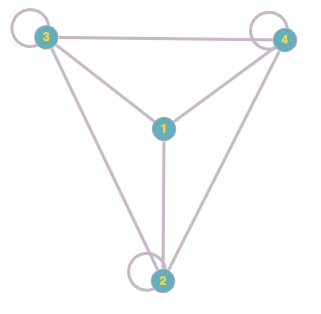
\includegraphics[width=0.35\linewidth]{figs/graphs/graph_A.png}
%     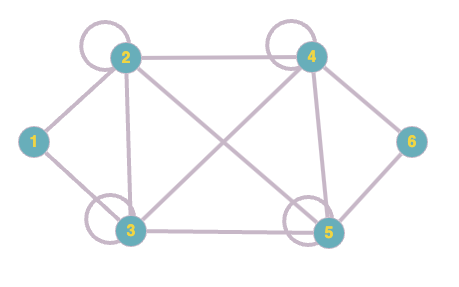
\includegraphics[width=0.425\linewidth]{figs/graphs/graph_B.png}
%     \caption{Fundamental graphs used for levels 3 (left) and 4 (right).}
%     \label{fig:graphs}
% \end{figure}

\begin{figure}
    \centering
    \begin{tikzpicture}
        \node[shape=circle,draw=black] (A) at (1.5,1.66) {1};
        \node[shape=circle,draw=black] (B) at (0,3) {2};
        \node[shape=circle,draw=black] (C) at (3,3) {3};
        \node[shape=circle,draw=black] (D) at (1.5,0) {4};
        
        \path (B) edge [loop, in=120, out=180, looseness=10] node {} (B);
        \path (C) edge [loop, in=0, out=60, looseness=10] node {} (C);
        \path (D) edge [loop, in=240, out=300, looseness=10] node {} (D);
        
        \path [-] (D) edge node {} (B);
        \path [-] (B) edge node {} (C);
        \path [-] (C) edge node {} (D);

        \path [-] (A) edge node {} (B);
        \path [-] (A) edge node {} (C);
        \path [-] (A) edge node {} (D);
    \end{tikzpicture}
    \begin{tikzpicture}
        \node[shape=circle,draw=black] (A) at (1.5,1.66) {1};
        \node[shape=circle,draw=black] (B) at (0,3) {2};
        \node[shape=circle,draw=black] (C) at (3,3) {3};
        \node[shape=circle,draw=black] (D) at (1.5,0) {4};

        \path [->] (A) edge [loop, in=45, out=135, looseness=8] node {} (A);

        \path [->] (B) edge node {} (C);
        \path [->] (C) edge node {} (D);
        \path [->] (D) edge node {} (B);
    \end{tikzpicture}
    \caption{Fusion graphs at level 3 for $Y$ (left) and $g$ (right).}
    \label{fig:new-graphs-lvl3}
\end{figure}


\begin{figure}
    \begin{tikzpicture}
        \node[shape=circle,draw=black] (A) at (0,1.5) {1};
        \node[shape=circle,draw=black] (B) at (1.25,3) {2};
        \node[shape=circle,draw=black] (C) at (4.25,3) {3};
        \node[shape=circle,draw=black] (D) at (5.5,1.5) {4};
        \node[shape=circle,draw=black] (E) at (4.25,0) {5};
        \node[shape=circle,draw=black] (F) at (1.25,0) {6};

        \path (B) edge [loop, in=45, out=135, looseness=8] node {} (B);
        \path (C) edge [loop, in=45, out=135, looseness=8] node {} (C);
        \path (E) edge [loop, in=225, out=315, looseness=8] node {} (E);
        \path (F) edge [loop, in=225, out=315, looseness=8] node {} (F);

        \path [-] (A) edge node {} (B);
        \path [-] (A) edge node {} (F);

        \path [-] (B) edge node {} (C);
        \path [-] (B) edge node {} (E);
        \path [-] (B) edge node {} (F);

        \path [-] (C) edge node {} (D);
        \path [-] (C) edge node {} (E);
        \path [-] (C) edge node {} (F);

        \path [-] (D) edge node {} (E);

        \path [-] (E) edge node {} (F);
    \end{tikzpicture}
    \begin{tikzpicture}
        \node[shape=circle,draw=black] (A) at (0,1.5) {1};
        \node[shape=circle,draw=black] (B) at (1.25,3) {2};
        \node[shape=circle,draw=black] (C) at (4.25,3) {3};
        \node[shape=circle,draw=black] (D) at (5.5,1.5) {4};
        \node[shape=circle,draw=black] (E) at (4.25,0) {5};
        \node[shape=circle,draw=black] (F) at (1.25,0) {6};

        \path [->] (A) edge [loop, in=135, out=225, looseness=8] node {} (A);
        \path [->] (D) edge [loop, in=45, out=-45, looseness=8] node {} (D);

        \path [->] (B) edge [bend right] node  {} (F);
        \path [->] (F) edge [bend right] node {} (B);

        \path [->] (C) edge [bend right] node {} (E);
        \path [->] (E) edge [bend right] node {} (C);
    \end{tikzpicture}
    \caption{Fusion graphs at level 4 for $Y$ (left) and $g$ (right).}
    \label{fig:new-graphs-lvl4}
\end{figure}


\begin{table}
    \centering
    \begin{tabular}{|cc|c|} \hline
        Vertex Path & Conditions & Coefficient \\ \hline\hline
        $(i,i,i)$ &  $i\neq1$ & 1.08393 \\[10pt]  \hline
        $(i,j,k)$ &  $\{i,j,k\}=\{2,3,4\}$   & 0.619371 \\[10pt] \hline
        $(i,1,k)$ &  $i,k\neq 1$, $i\neq k$ & 1.69414 \\[10pt] \hline
        $(i,1,i)$ &  $i\neq 1$   & 0.861006 \\[10pt] \hline
        $(i,i,1)$ or $(1,i,i)$ &  $i\neq1$   & 0.967919 \\[10pt] \hline
    \end{tabular}
    \caption{Level 3 trivalent embedding coefficients.}
    \label{tab:lvl-3-triv-coefs}
\end{table}






\begin{table}
    \centering
    \begin{tabular}{|cccc|} \hline
        $1\to\blank\to1$                    & $2\to\blank\to4$                  & $3\to\blank\to2$               & $4\to\blank\to3$ \\ \hline\hline
        $1.26376$              & $0.791288$                & $0.791288 $              & $0.791288$ \\
        $-0.631881-1.09445 i$   & $0.567622 - 0.684904 i$   & $0.876955 + 0.149123 i$  & $0.674406 + 0.580055 i$ \\
        $-0.631881+1.09445 i$   & $0.674406 + 0.580055 i$   & $0.567622 - 0.684904 i$  & $0.876955 + 0.149123 i$ \\
        $-0.631881+1.09445 i$   & $-0.876955 - 0.149123 i$  & $-0.674406 - 0.580055 i$ & $0.567622 - 0.684904 i$ \\
        $1.26376$               & $0.567622 + 0.684904 i$   & $0.876955 - 0.149123 i$ & $0.674406 - 0.580055 i$ \\
        $-0.631881-1.09445 i$   & $1$                       & $1$                      & $1$ \\
        $-0.631881-1.09445 i$   & $-0.0182917 + 0.999833 i$ & $0.5 - 0.866025 i$       & $0.856735 - 0.515757 i$ \\
        $-0.631881+1.09445i$    & $-0.5 - 0.866025 i$       & $-0.856735 - 0.515757 i$ & $-0.0182917 - 0.999833 i$ \\
        $1.26376$               & $0.674406 - 0.580055 i$   & $0.567622 + 0.684904 i$  & $0.876955 - 0.149123 i$ \\ 
                              & $-0.0182917 - 0.999833 i$ & $0.5 + 0.866025 i$       & $0.856735 + 0.515757 i$ \\
                              & $1$                       & $1$                      & $1$ \\
                              & $-0.856735 + 0.515757 i$  & $0.0182917 - 0.999833 i$ & $0.5 - 0.866025 i$ \\
                              & $-0.876955 + 0.149123 i$  & $-0.674406 + 0.580055 i$ & $0.567622 + 0.684904 i$ \\
                              & $-0.5 + 0.866025 i$       & $-0.856735 + 0.515757 i$ & $-0.0182917 + 0.999833 i$ \\
                              & $-0.856735 - 0.515757 i$  & $0.0182917 + 0.999833 i$ & $0.5 + 0.866025 i$ \\
                              & $1$                       & $1$                      & $1$ \\ \hline
    \end{tabular}
    \caption{Level 3 projection embedding coefficients.}
    \label{tab:lvl-3-proj-coefs}
\end{table}




Finally we give explicit values for the coefficients of the equations of Proposition~\ref{prop:eval-criteria}, excluding (decTetragon) and (decPentagon); the curious reader may find these in the attached Mathematica notebook. The structure constants for $\DD_3$ are:
\begin{equation*}
    \omega = e^{2\pi i/3}
\end{equation*}

\begin{equation*}
    r_1 = ..., \quad r_2 = ..., \quad r_3 = ...
\end{equation*}

\begin{equation*}
    s_1 = ..., \quad s_2 = ..., \quad s_3 = ...
\end{equation*}

\begin{equation*}
    r_1 = ..., \quad r_2 = ..., \quad r_3 = ...
\end{equation*}

\begin{equation*}
    t_1 = ..., \quad t_2 = ..., \quad t_3 = ...
\end{equation*}




\subsection{Theorem and proof}
This subsection is devoted to proving the following theorem.

\begin{theorem}\label{thm:level-3}
    There is a monoidal equivalence
    \[
        \Ab(\ol{\DD_3}) \cong \ol{ \Rep(U_{q_3}(\gg_2))}_{A_3}.
    \]
\end{theorem}

Let $X = V_{\Lambda_1}$ be the object of $\cat{q_3}$ by which we generate the planar algebra $\PP_X \cong \GG_2(q)$. Define $Y=\FF_A(X)$ to be the image of $X$ under the free functor. Now $\FF_{A_3}:\cat{q_3} \to \cat{q_3}_{A_3}$ restricts to an embedding $\PP_{X;\cat{q_3}} \hookrightarrow \PP_{Y;\cat{q}_{A_3}}$. Invertibility of the objects $g$ and $g^{-1}$ implies $g\otimes Y \cong Y$, with rigidity maps for $g$ and $g^{-1}$ building the mutually inverse isomorphisms.

We now compute some important dimensions.
\begin{proposition}\label{prop:level-3-fusion}
    The following are true:
    \begin{enumerate}
        \item $\dim\Hom_{\CC_{A_3}}(Y^{\otimes2}\to Y)=3$
        \item $\dim\Hom_{\CC_{A_3}}(Y^{\otimes2}\to g^k)=1$
        \item $\dim\Hom_{\CC_{A_3}}(Y\to Y)=1$ (i.e., $Y$ is simple)
    \end{enumerate}
\end{proposition}
\begin{proof}
    All three are proved using fusion graph calculations, so we prove only (1)\footnote{See, e.g., Figure 5 of \cite{spectral_measures_G2} for the fusion graph.}. The fusion graph tells us that 
    \[
    V_{\Lambda_1}^{\otimes2} \cong V_\emptyset \oplus V_{\Lambda_1} \oplus V_{2\Lambda_1} \oplus V_{\Lambda_2}
    \]
    and
    \[
    V_{\Lambda_1}\otimes A \cong V_{\Lambda_1} \oplus V_{2\Lambda_1} \oplus  V_{3\Lambda_1} \oplus V_{\Lambda_2} \oplus V_{\Lambda_2+\Lambda_1} \oplus V_{\Lambda_2+2\Lambda_1}.
    \]
    On the other hand, we compute
    \begin{align*}
        \Hom_{\cat{q_3}_{A_3}}(Y^{\otimes2} \to Y) & = \Hom_{\CC_{A_3}}( \FF_{A_3}(V_7)^{\otimes 2} \to \FF_{A_3}(V_7)) \\
        & \cong \Hom_{\cat{q_3}_{A_3}}( \FF_{A_3}(V_7^{\otimes 2}) \to \FF_{A_3}(V_7)) \\
        & = \Hom_{\cat{q_3}_{A_3}}( \FF_{A_3}(V_7^{\otimes 2}) \to V_7\otimes {A_3}) \\
        & \cong \Hom_{\cat{q_3}}( V_7^{\otimes 2} \to V_7\otimes {A_3}). \\
    \end{align*}
    Counting common irreducible constituents of $V_{\Lambda_1}^{\otimes2}$ and $V_{\Lambda_1}\otimes A_3$ gives the desired result.
\end{proof}
We have an immediate consequence.
\begin{corollary}\label{cor:dominant-functor}
        There is a dominant monoidal functor
    \[
        \Psi_3: \DD_3 \to \cat{q}_{A_3}
    \]
    which maps 
    \[
        \skein{/skein_figs/trivalent}{0.15} \mapsto \tau\in\Hom_{\cat{q_3}_{A_3}}(Y^{\otimes2}\to Y), \quad \skein{/skein_figs/Pg}{0.15} \mapsto P_g \in\End_{\cat{q_3}_{A_3}}(Y^{\otimes2})
    \]
\end{corollary}
\begin{proof}
    Proposition~\ref{prop:level-3-fusion}, along with the defining relations of $\DD_3$ tell us this assignment is functorial. 
    Since $Y$ is a $\otimes$-generator and $\Psi_3$ surjects onto objects of $\PP_Y$, dominance also follows.
\end{proof}




\begin{lemma}\label{lem:faithful}
    The induced map
    \[
        \ol{\Psi_3} : \ol{\DD_3} \to \ol{\Rep(U_{q_3}(\gg_2))}_{A_3} 
    \]
    is faithful.
\end{lemma}
% Why do we care...?
\begin{proof}
    The evaluation algorithm for $\DD_3$ implies that $\DD_3$ has simple unit. Therefore every ideal is contained in the ideal of negligibles, which is killed when passing to the semisimplification $\ol{\DD}$. Hence the map $\ol{\Psi_3}$ has no kernel.
\end{proof}

\begin{proof}[Proof of Theorem~\ref{thm:level-3}]
    We now note that since $\GG_2(q)$ and $\DD_3$ are unitary, we know that $\GG_2(q) \hookrightarrow \DD_3$ induces a $\dagger$-embedding $\ol{\GG_2(q)} \hookrightarrow \ol{\DD_3}$. Thus, there is a chain
    \[
        \ol{\GG_2(q_3)} \hookrightarrow \ol{\DD_3} \xhookrightarrow{\ol{\Psi_3}} \ol{\Rep(U_{q_3}(\gg_2))}_{A_3}
    \] 
    of faithful dominant functors. Using the universal property of Karoubi completion, we arrive at the commutative diagram
    \[
        \xymatrix@R=40pt@C=65pt{
        \ol{\GG_2(q_3)} \ar@{^{(}->}[r] \ar@{^{(}->}[d] & \ol{\DD_3} \ar@{^{(}->}[dr]^{\ol{\Psi}} \ar@{^{(}->}[d] & \\
        \ol{\Rep(U_{q_3}(\gg_2))} \ar[r]^{\FF_1} & \Ab(\ol{\DD_3}) \ar[r]^{\FF_2} & \ol{\Rep(U_{q_3}(\gg_2))}_{A_3} \\
        }
    \]
    where $\FF_1$ and $\FF_2$ are the induced functors. At this point we shift our focus to the lower layer of the diagram.
    
    By \cite{},  $(\FF_2 \circ \FF_1)|_{\ol{\GG_2(q_3)}} = \FF_{A_3}|_{\ol{\GG_2(q_3)}}$ implies $\FF_2 \circ \FF_1 = \FF_{A_3}$. 
    Note that both $\ol{\Rep(U_{q_3}(\gg_2))}$ and $\Ab(\ol{\DD_3})$ are semisimple, and therefore $\FF_1$ has a lax-monoidal right adjoint $\FF_1^\vee$. 
    Proposition~\ref{prop:exact-functor} now allows us to conjure $K$ and $B$ such that the following diagram commutes up to natural isomorphism:
    \[
        \xymatrix@R=40pt@C=65pt{
        \ol{\Rep(U_{q_3}(\gg_2))} \ar[r]^{\FF_1} \ar[dr]_{\FF_B} & \Ab(\ol{\DD_3}) \ar[r]^{\FF_2} \ar[d]^{K} & \ol{\Rep(U_q(\gg_2))}_A \\
        & \ol{\Rep(U_q(\gg_2))}_B \ar[ur]_{\FF'} & \\
        }
    \]
    Here, $\FF'$ is defined to complete the diagram. From here, apply $\FF_B^\vee$ to the containment $\unit \subseteq \FF'^\vee(\unit)$:
    \begin{align*}
        B & = \FF_B^\vee(\unit) \subseteq \FF_B^\vee \circ \FF'^\vee(\unit) \\
        & \cong (\FF_2 \circ \FF_1)^\vee (\unit) \\
        & = \FF_{A_3}^\vee(\unit) \\
        & = \FF_A^\vee(A_3) = A_3.
    \end{align*}
    
    So $B\subseteq A_3$. Since $A_3$ has only two simple summands, we know $A_3$ has no nontrivial subalgebras: $B\cong \unit$ or $B\cong A_3$.
    If $B\cong \unit$ then
    \[
        \Ab(\ol{\DD_3}) \cong \ol{\Rep(U_{q_3}(\gg_2))}_\unit \cong \ol{\Rep(U_{q_3}(\gg_2))}
    \]
    A quick dimension count falsifies this. Hence $\Ab(\ol{\DD_3}) \cong \ol{ \Rep(U_{q_3}(\gg_2))}_{A_3}$.
\end{proof}








\section{Results: Level 4}
At level $k=4$ we have $q = q_4 = e^{\frac{2\pi i}{48}}$ and 
$A_4=V_\emptyset \oplus V_{3\Lambda_1}$. 
From \cite{DMNO} we have $\cat{q_4}_{A_4}^0 \cong \Vecc(\Z_2)$, giving us one new 
$\Z_2$-like simple object $h$. 
The details of the GPA embedding at level 4 are less instructive than the level 3 case, 
so we relegate the details to the attached Mathematica files. 
Much of the story remains the same. 
The trivalent coordinates are algebraically nicer than those at level 3; 
up to sign, we showed 5 of 9 in Subsection~\ref{subsec:triv-vertex}. 
The nonzero coordinates of the projection come in blocks of \red{4, and 9}. 
There is also an analogue of Theorem~\ref{thm:level-3} for level 4.

\begin{theorem}\label{thm:level-4}
    There is a monoidal equivalence
    \[
        \Ab(\ol{\DD(q_4)}) \cong \ol{ \Rep(U_{q_4}(\gg_2))}_{A_4}.
    \]
\end{theorem}

This theorem is proved by using analogues of Proposition~\ref{prop:level-3-fusion}, Corollary~\ref{cor:dominant-functor}, Lemma~\ref{lem:faithful}.
The same argument used in the proof of Theorem~\ref{thm:level-3} except with, e.g., every $q_3$ switched out for a $q_4$, may be applied.

Note that since $\cat{q_4}_{A_4}^0$ contributes a $\Z_2$-like simple object, there is only one decoration of a trivalent vertex;
we represent this as an undirected colored strand.
The structure constants for $\DD_4$ are:
\begin{equation*}
    \omega = -1
\end{equation*}

\begin{equation*}
    r_1 = -1, \quad r_2 = -1
\end{equation*}

\begin{equation*}
    s_1 = ..., \quad s_2 = ...
\end{equation*}

\begin{equation*}
    r_1 = ..., \quad r_2 = ...
\end{equation*}

\begin{equation*}
    t_1 = ..., \quad t_2 = ...
\end{equation*}



\printbibliography

\end{document}
